%\RequirePackage{lineno}

\documentclass[aps,prc,preprint,superscriptaddress,showpacs,showkeys,amsmath]{revtex4-1}
%\documentclass[article,showpacs,preprintnumbers,amsmath,amssymb]{revtex4}
\usepackage{graphicx}
\usepackage[usenames,dvipsnames,svgnames,table]{xcolor}
\usepackage{rotating}
\usepackage{graphicx}% Include  files
\usepackage{dcolumn}% Align table columns on decimal point
\usepackage{bm}% bold math
\usepackage{epsfig}
\usepackage{hyperref}
\usepackage{ulem}

\begin{document}

\newcommand{\Jpsi}{J/\psi}
\newcommand{\pT}{p_{T}}
\newcommand{\calO}{{\cal{O}}}
\newcommand{\barQ}{{\bar{Q}}}
\newcommand{\barc}{{\bar{c}}}
\newcommand{\barb}{{\bar{b}}}
\newcommand{\baru}{\bar{u}}
\newcommand{\barv}{\bar{v}}
\newcommand{\barup}{\bar{u}_{+}}
\newcommand{\barum}{\bar{u}_{-}}
\newcommand{\barvp}{\bar{v}_{+}}
\newcommand{\barvm}{\bar{v}_{-}}

%\linenumbers
\title{{\Large Quarkonia production and dissociation in Pb+Pb collisions}} 
\author{\large Vineet Kumar}
\author{\large Prashant Shukla}
\email{pshukla@barc.gov.in}
\affiliation{Nuclear Physics Division, Bhabha Atomic Research Center, Mumbai, India}
\affiliation{Homi Bhabha National Institute, Anushakti Nagar, Mumbai, India}
%\author{\large Ramona Vogt}
%\affiliation{Nuclear and Chemical Sciences Division, Lawrence Livermore National Laboratory, Livermore, CA 94551, USA}
%\affiliation{Physics Department, University of California, Davis, CA 95616, USA}

\date{\today}

\begin{abstract}
  We calculate the high p$_{T}$ quarkonia production using NRQCD method.
  Different methods of quarkonia suppression are used to explain the high
  p$_{T}$ quarkonia suppression obseved by CMS in LHC
\end{abstract}

\pacs{12.38.Mh, 24.85.+p, 25.75.-q}
\keywords{quark-gluon plasma, quarkonia, suppression, regeneration}

\maketitle

%%%%%%%%%%%%%%%%%%%%%%%%%%%%%%%%%%%%%%%%%%%%%%%%%%%%%%%%%%%%%%%%%%%%%%%%%%%%%%%%%%%%%%%%%%%%%%%%%%%%%%%%%%%%%%%%%
\section{Introduction}
Heavy-ion collisions at relativistic energies are performed to create and characterize 
quark gluon plasma (QGP), a phase of strongly-interacting matter at high energy density 
where quarks and gluons are no longer bound within hadrons.
The quarkonia states ($\Jpsi$ and $\Upsilon$) have been some of the most popular tools 
since their suppression was proposed as a signal of QGP formation \cite{Matsui:1986dk}.
The understanding of these probes has evolved substantially via measurements 
through three generations of experiments: the SPS (at CERN), RHIC (at BNL) and the LHC (at CERN) 
and by a great deal of theoretical activity. (For recent reviews see 
Refs.~\cite{Schukraft:2013wba,Kluberg:2009wc,Brambilla:2010cs}.)
Quarkonia are produced early in the heavy-ion collisions and, if they evolve
through the deconfined medium, their yields should be suppressed in comparison with those in $pp$ collisions. 
The first such measurement was the `anomalous' $\Jpsi$ suppression discovered at the SPS 
which was considered to be a hint of QGP formation. The RHIC measurements showed almost the 
same suppression at a much higher energy contrary to expectation \cite{Brambilla:2010cs,Adare:2011yf}. 
Such an observation was consistent with the scenario that, at higher collision energies, the 
expected greater suppression is compensated by  $\Jpsi$ regeneration through recombination of two 
independently-produced charm quarks~\cite{Andronic:2003zv}. 

In this paper, we calculate $\Jpsi$ and $\Upsilon$ production and
suppression 

\begin{figure}
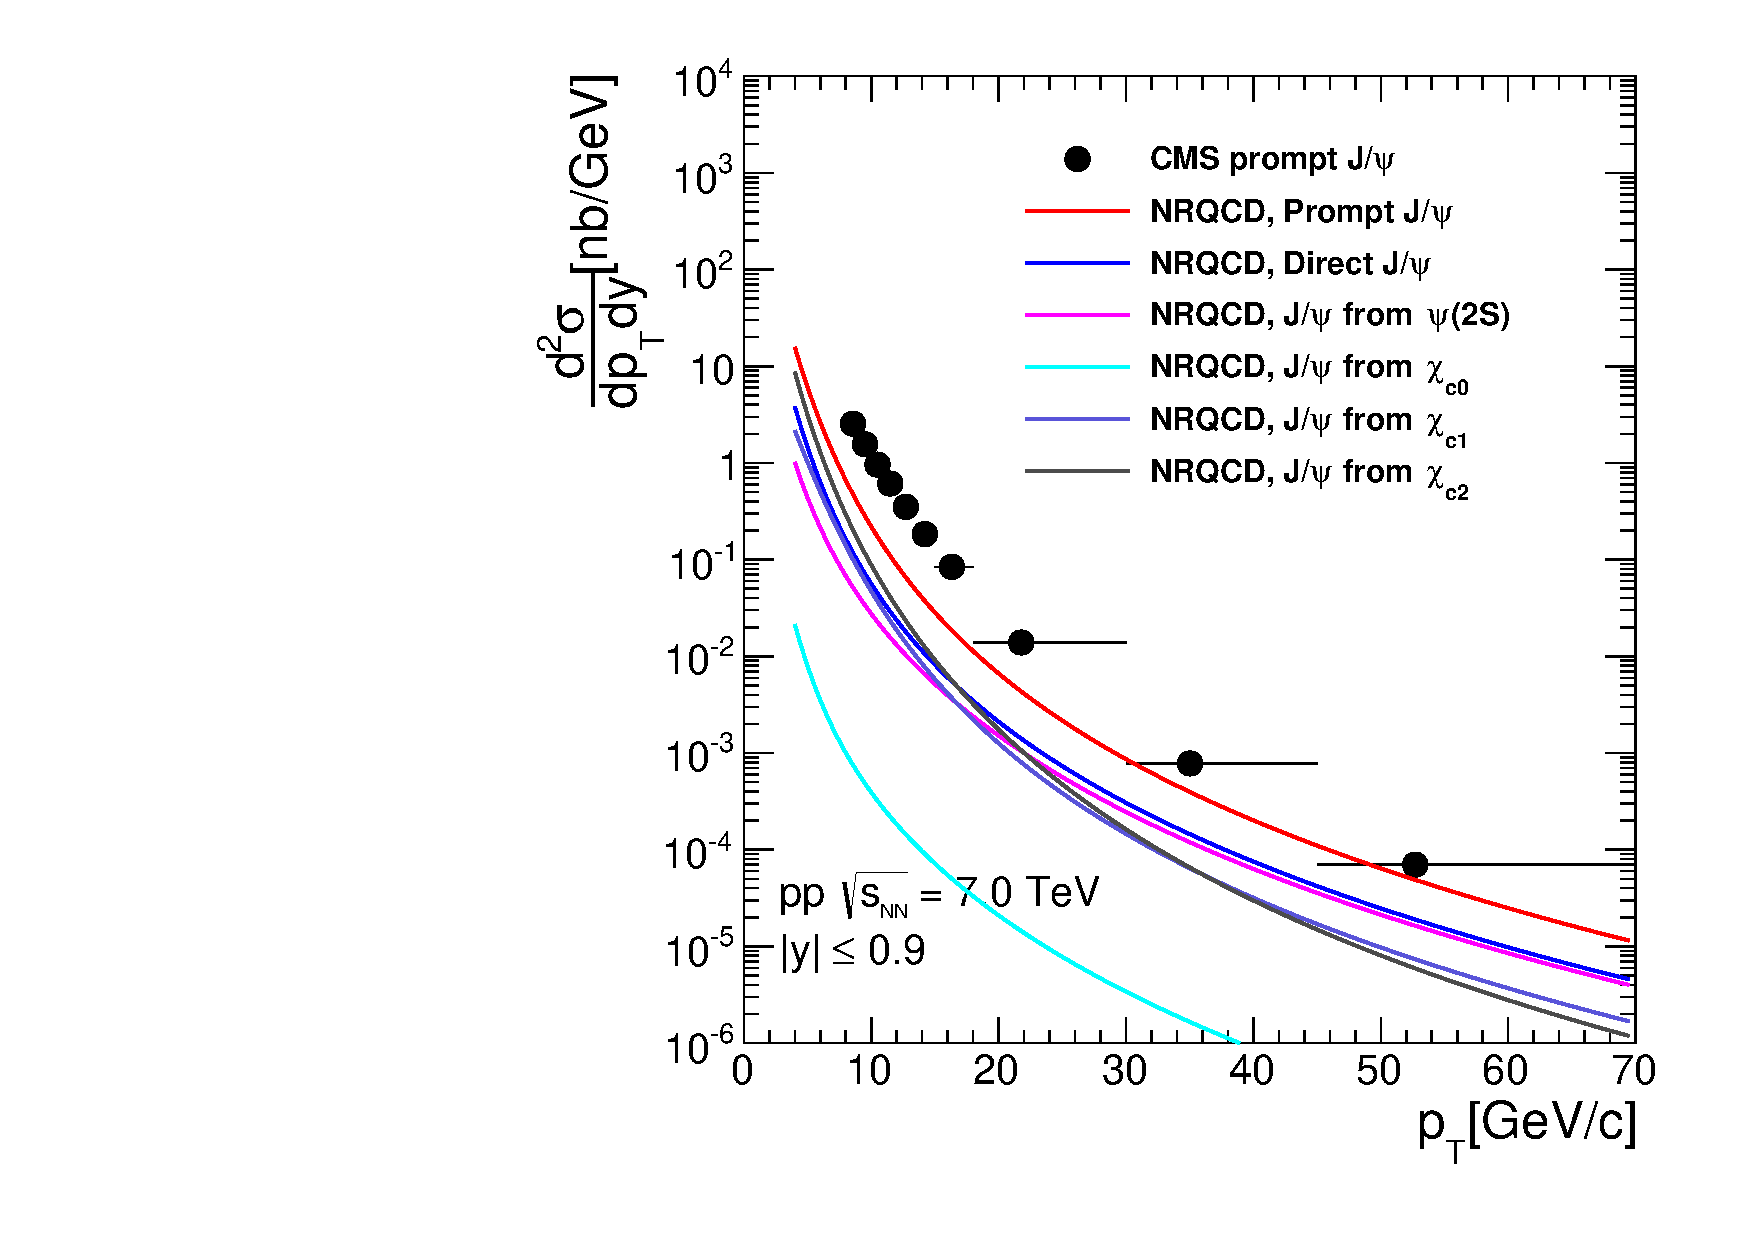
\includegraphics[width=0.49\textwidth]{Fig1a_JPsi_CMS_Y09_S7TeV.pdf}
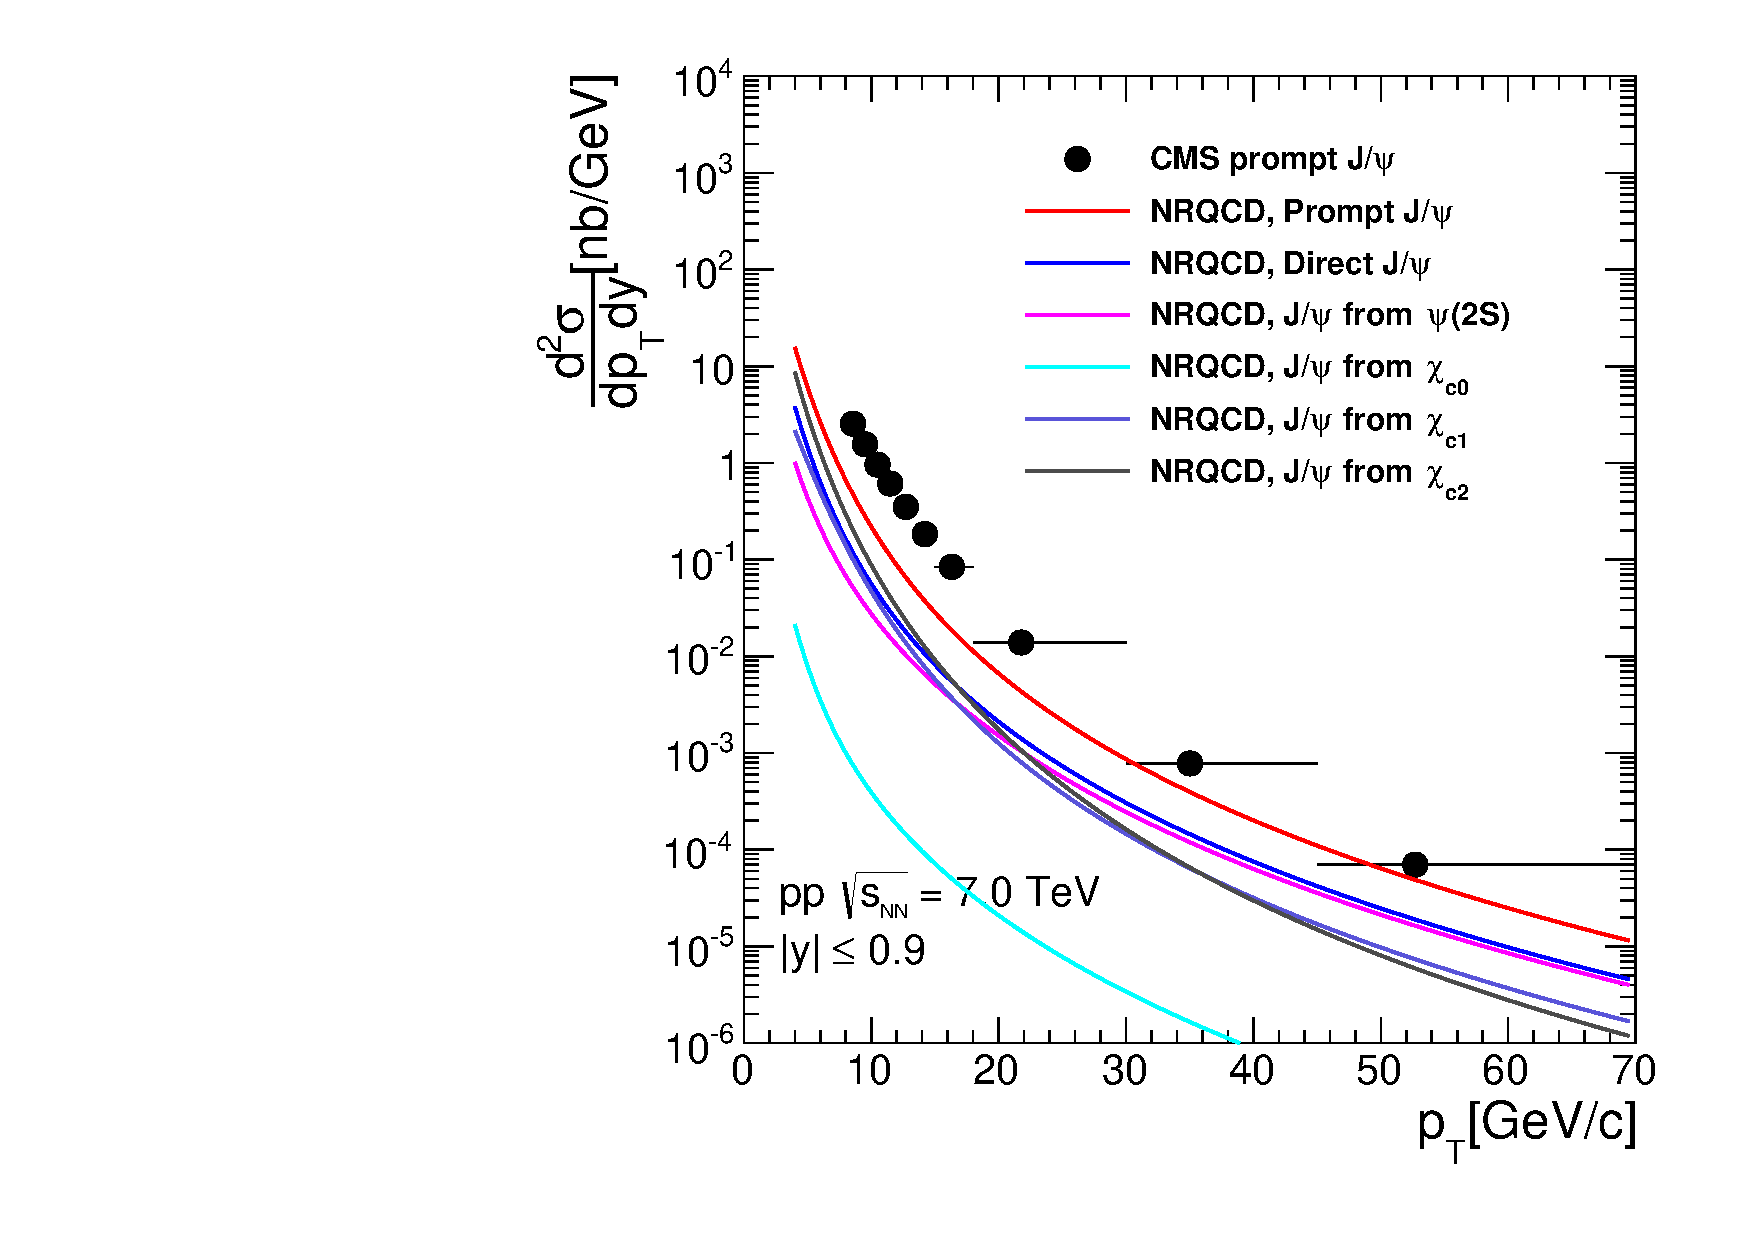
\includegraphics[width=0.49\textwidth]{Fig1a_JPsi_CMS_Y09_S7TeV.pdf}
\caption{(Color online) Differential production cross-section of $J/\psi$ as a function of $p_{T}$ compared 
  with the CMS~\cite{jhep02} data.}
\label{fig:TauVsTemp}
\end{figure}


%%%%%%%%%%%%%%%%%%%%%%%%%%%%%%%%%%%%%%%%%%%%%%%%%%%%%%%%%%%%%%%%%%%%%%%%%%%%%%%%%%%%%%%
\section{Quarkonia Production in p$+$p collisions}
\label{section:ppProduction}
In this section we describe the production of quarkonia at high transverse
momenta in p$+$p collisions. 

The factorization formalism of the NRQCD  provides a theoretical framework for studying the heavy quarkonium production and decay. 
According to the NRQCD factorization  formalism, the cross-section for direct production of a resonance $H$ in a collision of 
particle $A$ and $B$ can be expressed as 
\begin{equation}
  d\sigma_{A+B\rightarrow H+X} = \sum_{a,b,n}\int dx_a dx_b  G_{a/A}(x_a,\,\mu^{2}_{F})\, G_{b/B}(x_b,\,\mu^{2}_{F})
  \times d\sigma(a+b\rightarrow Q\bar Q(n) +X)<\mathcal{O}^H(n)>
\end{equation}
where, $G_{a/A}(G_{b/B})$ is the parton distribution function (PDF) of the incoming parton $a(b)$ in the incident hadron $A(B)$, which depends on 
the momentum fraction $x_a(x_b)$ and the factorization scale $\mu_F$ as well as on the renormalization scale $\mu_R$. However, 
as we have chosen $\mu_F$ = $\mu_R$, in our case PDFs are function of $x$ and $\mu_F$ only. The tranverse mass of the 
resonance $H$ is $m_T = \sqrt{p_T^2 + m_H^2}$, where $m_H\sim2m_Q$ is the mass of resonance $H$. The short distance 
contribution $d\sigma(a+b\rightarrow Q\bar Q(n) +X)$ can be calculated within the framework of perturbative QCD (pQCD). 
On the other hand, $<\mathcal{O}^H(n)>$ (the state $n=^{2S+1}L^{[i]}_J$) are nonperturbative LDMEs and can be estimated on the basis of 
the comparison with experimental measurements. 

The dominant processes in evaluating the differential 
yields of heavy mesons as a function of $p_T$ are the $2\rightarrow 2$
processes of the kind $g+q\rightarrow H+q$, $q+\bar{q}\rightarrow H+g$ and
$g+g\rightarrow H+g$, where $H$ refers to the heavy meson. We label the process
generically as $a+b\rightarrow c+d$, where $a$ and $b$ are light incident
partons, $c$ refers to $H$ and $d$ is a light final-state parton. The differential cross-section 
for the short distance contribution i.e. the heavy quark pair production 
from the reaction of the type $a\,+\,b\,\rightarrow\,c\,+\,d$ can be written as~\cite{Owens:1986mp}

\begin{equation}
  \frac{{d\sigma}^{ab\rightarrow cd}}{dp_T\,dy} = \int dx_a\, G_{a/A}(x_a,\,\mu^{2}_{F})\, G_{b/B}(x_b,\,\mu^{2}_{F})\times 
  2p_T \frac{x_a\,x_b}{x_a-\frac{m_T}{\sqrt{s}}e^y}\frac{d\sigma}{d\hat t}(ab\rightarrow cd),
\end{equation}

where, $\sqrt{s}$ being the total energy in the centre-of-mass and $y$ is the rapidity of 
the $Q\bar Q$ pair. In our numerical computation, we use CTEQ6M~\cite{Lai:2010vv} for the parton 
distribution functions. The invariant differential cross-section is given by
\begin{equation}
\frac{d\sigma}{d\hat t} = \frac{|\mathcal{M}|^2}{16\pi{\hat s}^2},
\end{equation}
where $\hat s$ and $\hat t$ are the parton level Mandelstam variables. $\mathcal{M}$ is the 
feynman amplitude for the process. Energy momentum conservation fixes value of the momentum 
fraction $x_b$ as,
\begin{equation}
x_b = \frac{1}{\sqrt{s}}\frac{x_a\,\sqrt{s}\,m_T\,e^{-y}-m^2_H}{x_a\,\sqrt{s}-m_T\,e^y}.
\end{equation}

The minimum value of $x_a$ is 
\begin{equation}
x_{a\rm min} = \frac{1}{\sqrt{s}}\frac{\sqrt{s}\,m_T\,e^{y}-m^2_H}{\sqrt{s}-m_T\,e^{-y}}.
\end{equation}

The LDMEs are predicted to scale with a definite power of the relative velocity $v$ of the heavy constituents inside $Q\bar Q$ bound states. 
In the limit $v<<1$, the production of quarkonium is based on the $^3S_1^{[1]}$ and $^3P_J^{[1]}$ ($J$ = 0,1,2) CS states 
and $^1S_0^{[8]}$, $^3S_1^{[8]}$ and $^3P_J^{[8]}$ CO states. In our calculations, we used the expressions for the short distance CS cross-sections 
given in Refs.~\cite{Baier:1983va,Gastmans:1987be} and the CO cross-sections given in Refs.~\cite{Cho:1995vh,Cho:1995ce}.

In this section we calculate the $p_T$ distribution of $J/\psi$, $\psi(2S)$ and $\Upsilon$(nS) mesons in $p-p$ collisions 
at LHC energies. For $J/\psi$ production in $p-p$ collisions, three sources need to be considered: 
direct $J/\psi$ production, feed-down contributions to the $J/\psi$ from the decay of heavier charmonium states, 
predominantly from $\psi(2S)$, $\chi_{c0}$, $\chi_{c1}$ and $\chi_{c2}$ and $J/\psi$ 
from $B$ hadron decays. The sum of the first two sources is called "prompt $J/\psi$" and the third source will be called "$J/\psi$ from $B$". 
On the other hand, $\psi(2S)$ has no significant feed-down contributions from higher mass states. We call this direct contribution as 
"prompt $\psi(2S)$" to be consistent with the experiments. The other source to $\psi(2S)$ production is from $B$ hadron decays and
 we call it "$\psi(2S)$ from $B$". The sum of the prompt $J/\psi$($\psi(2S)$) and $J/\psi$($\psi(2S)$) from $B$ will be called 
"inclusive $J/\psi$($\psi(2S)$)". Similar terminology is used for $\Upsilon$ states, only differnce is that we do not have 
any contribution from open T mesons.

NRQCD provides a systematic procedure to compute any quantity as an expansion in the relative velocity $v$
of the heavy quarks in the meson. For example, the wavefunction of the $J/\psi$
meson (analogous expressions hold for the $\psi(2S)$, $\Upsilon(1S)$,
$\Upsilon(2S)$ and $\Upsilon(3S)$) is written as

\begin{equation}
\begin{split}
|J/\psi\rangle = &|Q\barQ([^3S_1]_{1})\rangle 
+ \calO(v)|Q\barQ([^1S_0]_{8}g)\rangle 
  + \calO(v^2)|Q\barQ([^3S_1]_{8}gg)\rangle\\
  &+ \calO(v^1)|Q\barQ([^3P_0]_{8}g)\rangle
  + \calO(v^1)|Q\barQ([^3P_1]_{8}g)\rangle
  + \calO(v^1)|Q\barQ([^3P_2]_{8}g)\rangle
  +\cdot\cdot\cdot
  \label{eq:Jfock}
\end{split}
\end{equation}

The differential cross section for the direct production of $J/\psi$ can be written 
as the sum of the contributions,
\begin{equation}
\begin{split}
d\sigma(J/\psi) &= d\sigma(Q\barQ([^3S_1]_{1}))
                  \langle \calO(Q\barQ([^3S_1]_{1})\rightarrow J/\psi)\rangle 
                +  d\sigma(Q\barQ([^1S_0]_{8}))
                  \langle \calO(Q\barQ([^1S_0]_{8})\rightarrow J/\psi)\rangle\\ 
                &+  d\sigma(Q\barQ([^3S_1]_{8}))
                  \langle \calO(Q\barQ([^3S_1]_{8})\rightarrow J/\psi)\rangle 
                +  d\sigma(Q\barQ([^3P_0]_{8}))
                  \langle \calO(Q\barQ([^3P_0]_{8})\rightarrow J/\psi)\rangle\\ 
                &+  d\sigma(Q\barQ([^3P_1]_{8}))
                  \langle \calO(Q\barQ([^3P_1]_{8})\rightarrow J/\psi)\rangle
                +  d\sigma(Q\barQ([^3P_2]_{8}))
                  \langle \calO(Q\barQ([^3P_2]_{8})\rightarrow J/\psi)\rangle
                + \cdot\cdot\cdot  \;,
\label{eq:dsigmaJ}
\end{split}
\end{equation}
where the quantity in the brackets $[\;]$ represents the angular momentum
quantum numbers of the $Q\barQ$ pair in the Fock expansion. The subscript on
$[\;]$ refers to the color structure of the $Q\barQ$ pair, $1$ being 
the color-singlet and $8$ being the color-octet. The dots represent terms which contribute at
higher powers of $v$. The short distance cross sections $d\sigma(Q\barQ)$
correspond to the production of a $Q\barQ$ pair in a particular color and spin
configuration, while the long distance matrix element
$\langle\calO(Q\barQ)\rightarrow J/\psi\rangle$ corresponds to the probability
of the $Q\barQ$ state to convert to the quarkonium wavefunction. This
probability includes any necessary prompt emission of soft gluons to prepare a
color neutral system that matches onto the corresponding Fock component of the
quarkonium wavefunction. 





\section{Summary}
 
 


 \section{Acknowledgement}
  The authors thank their CMS colleagues for the fruitful discussions, 
help and comments. Many of these results were presented at WHEPP and we acknowledge discussions 
with the participants of the meeting, in particular with D. Das, S. Datta, R. Gavai, S. Gupta
and R. Sharma. The work of RV was performed under the auspices of the US Department of Energy, 
Lawrence Livermore National Laboratory, Contract DE-AC52-07NA27344.


\noindent
\begin{thebibliography}{100}
\medskip

\bibitem{Matsui:1986dk} 
 T.~Matsui and H.~Satz,
 ``$J/\psi$ Suppression by Quark-Gluon Plasma Formation'',
 Phys.\ Lett.\ B {\bf 178}, 416 (1986).

\bibitem{Schukraft:2013wba} 
  J.~Schukraft,
  ``Heavy Ion Physics at the LHC: What's new ? What's next ?'',
  arXiv:1311.1429 [hep-ex].


\bibitem{Kluberg:2009wc} 
  L.~Kluberg and H.~Satz,
  ``Color Deconfinement and Charmonium Production in Nuclear Collisions,''
  arXiv:0901.3831 [hep-ph].

\bibitem{Brambilla:2010cs} 
  N.~Brambilla, S.~Eidelman, B.~K.~Heltsley, R.~Vogt, G.~T.~Bodwin, E.~Eichten, A.~D.~Frawley and A.~B.~Meyer {\it et al.},
  ``Heavy quarkonium: progress, puzzles, and opportunities,''
  Eur.\ Phys.\ J.\ C {\bf 71}, 1534 (2011).
  %[arXiv:1010.5827 [hep-ph]].

\bibitem{Adare:2011yf} 
  A.~Adare {\it et al.}  [PHENIX Collaboration],
  ``$J/\psi$ suppression at forward rapidity in Au+Au collisions at $\sqrt{s_{NN}}=200$ GeV,''
  Phys.\ Rev.\ C {\bf 84}, 054912 (2011).
  %[arXiv:1103.6269 [nucl-ex]].

\bibitem{Andronic:2003zv} 
  A.~Andronic, P.~Braun-Munzinger, K.~Redlich and J.~Stachel,
  ``Statistical hadronization of charm in heavy ion collisions at SPS, RHIC and LHC,''
  Phys.\ Lett.\ B {\bf 571}, 36 (2003).
 % [nucl-th/0303036].

%\cite{Owens:1986mp}
\bibitem{Owens:1986mp} 
  J.~F.~Owens,
  ``Large Momentum Transfer Production of Direct Photons, Jets, and Particles,''
  Rev.\ Mod.\ Phys.\  {\bf 59}, 465 (1987).
  %%CITATION = RMPHA,59,465;%%
  %531 citations counted in INSPIRE as of 16 Jun 2015

%\cite{Lai:2010vv}
\bibitem{Lai:2010vv} 
  H.~L.~Lai, M.~Guzzi, J.~Huston, Z.~Li, P.~M.~Nadolsky, J.~Pumplin and C.-P.~Yuan,
  ``New parton distributions for collider physics,''
  Phys.\ Rev.\ D {\bf 82}, 074024 (2010),
  [arXiv:1007.2241 [hep-ph]].
  %%CITATION = ARXIV:1007.2241;%%
  %1298 citations counted in INSPIRE as of 16 Jun 2015

%
\bibitem{Baier:1983va} 
  R.~Baier and R.~Ruckl,
  ``Hadronic Collisions: A Quarkonium Factory,''
  Z.\ Phys.\ C {\bf 19}, 251 (1983).
  %%CITATION = ZEPYA,C19,251;%%
  %436 citations counted in INSPIRE as of 16 Jun 2015



\bibitem{Gastmans:1987be} 
  R.~Gastmans, W.~Troost and T.~T.~Wu,
  ``Production of Heavy Quarkonia From Gluons,''
  Nucl.\ Phys.\ B {\bf 291}, 731 (1987).
  %%CITATION = NUPHA,B291,731;%%
  %94 citations counted in INSPIRE as of 16 Jun 2015



%\cite{Cho:1995vh}
\bibitem{Cho:1995vh} 
  P.~L.~Cho and A.~K.~Leibovich,
  ``Color octet quarkonia production,''
  Phys.\ Rev.\ D {\bf 53}, 150 (1996),
  [hep-ph/9505329].
  %%CITATION = HEP-PH/9505329;%%
  %409 citations counted in INSPIRE as of 16 Jun 2015

%\cite{Cho:1995ce}
\bibitem{Cho:1995ce} 
  P.~L.~Cho and A.~K.~Leibovich,
  ``Color octet quarkonia production. 2.,''
  Phys.\ Rev.\ D {\bf 53}, 6203 (1996),
  [hep-ph/9511315].
  %%CITATION = HEP-PH/9511315;%%
  %395 citations counted in INSPIRE as of 16 Jun 2015







\end{thebibliography}
\end{document}



